\documentclass{llncs}

\usepackage{ifxetex}
\ifxetex
\else
\usepackage[utf8]{inputenc}
\fi

\usepackage{amsmath}
\usepackage{mathcomp,amsfonts,amssymb}
\usepackage[mathscr]{euscript}
\usepackage{algorithmic,algorithm}
\usepackage{paralist}
\usepackage{graphicx}
%\usepackage{color}
\usepackage{placeins}

\usepackage{enumitem}
\usepackage{dcolumn}

\usepackage{listings}
\lstset{language=C,mathescape=true,numbers=left,numbersep=0.8ex,tabsize=2,breaklines=true,basicstyle={\rm\fontfamily{phv}\small\selectfont}}

\usepackage{tikz}
\usetikzlibrary{arrows,automata,positioning}

\tikzstyle{state}=[circle,fill=black!25,minimum size=13pt,inner sep=0pt]
\tikzstyle{rstate}=[rectangle,fill=black!25,minimum size=13pt,inner sep=0pt]
\tikzstyle{transition}=[rectangle,semithick,draw=black!75,
  			  minimum size=4mm]
\tikzstyle{transition2}=[transition,rectangle,thick,dashed,
  			  minimum size=4mm]
\tikzstyle{PRstate}=[circle,double,draw,fill=blue!15,minimum size=13pt,inner sep=0pt]
\tikzstyle{polyhedra}=[blue!25,opacity=0.5,pattern=north west lines,pattern
color=blue]
\tikzstyle{line}=[black,thick]

\newcommand{\mytitle}{Succinct Representations for Abstract Interpretation}
\usepackage[pdftitle={\mytitle},pdfauthor={Julien Henry, David Monniaux, Matthieu Moy}]{hyperref}

\newcommand{\abstr}[1]{#1^\sharp}
\newcommand{\parts}[1]{\mathscr{P}(#1)}
\newcommand{\ZZ}{\mathbb{Z}}
\newcommand{\QQ}{\mathbb{Q}}
\newcommand{\RR}{\mathbb{R}}
\newcommand{\widening}{\mathop{\triangledown}}

\graphicspath{{figures/}{gnuplot/}}

% commentaires dans les algorithmes crees avec le package algorithmic
\renewcommand{\algorithmiccomment}[1]{ {\color{gray} // #1}}

\usepackage{ifthen}
\newboolean{draft}
%\setboolean{draft}{true}
\setboolean{draft}{false}

\ifthenelse{\boolean{draft}}{
  \newcommand{\avirer}[1]{{\color{red} #1}}
  \newcommand{\MM}[1]{{\color{blue} TODO(MM): #1}}
  \newcommand{\JH}[1]{{\color{teal} TODO(JH): #1}}
  \newcommand{\DM}[1]{{\color{violet} TODO(DM): #1}}
}{
  \newcommand{\avirer}[1]{}
  \newcommand{\MM}[1]{}
  \newcommand{\JH}[1]{}
  \newcommand{\DM}[1]{}
}

\title{\mytitle\thanks{\protect\raisebox{-0.5em}{\protect
\includegraphics[height=1.5em]{ASOPT_officiel_nb}} This work was partially funded by ANR project ``ASOPT''}}
\subtitle{Combined analysis algorithms and experimental evaluation}
\author{Julien Henry\inst{1}\inst{2} \and David Monniaux\inst{1}\inst{3} \and Matthieu Moy\inst{1}\inst{4}}

\institute{VERIMAG laboratory, Grenoble, France
\and Université Joseph Fourier
\and CNRS
\and Grenoble-INP}

\renewcommand{\baselinestretch}{1}
\setlength{\floatsep}{1.5ex plus 0.5ex}
\setlength{\textfloatsep}{1.5ex plus 0.5ex}

\begin{document}
\maketitle

\begin{abstract}
Abstract interpretation techniques can be made more precise by distinguishing
paths inside loops, at the expense of possibly exponential complexity. SMT-solving techniques and sparse representations of paths and sets of paths avoid this pitfall.

We improve previously proposed techniques for guided static analysis and the generation of disjunctive invariants by combining them with techniques for succinct representations of paths and symbolic representations for transitions based on static single assignment.

Because of the non-monotonicity of the results of abstract interpretation with widening operators, it is difficult to conclude that some abstraction is more precise than another based on theoretical local precision results. We thus conducted extensive comparisons between our new techniques and previous ones, on a variety of open-source packages.
\end{abstract}

\documentclass[preprint]{sigplanconf}

% The following \documentclass options may be useful:
%
% 10pt          To set in 10-point type instead of 9-point.
% 11pt          To set in 11-point type instead of 9-point.
% authoryear    To obtain author/year citation style instead of numeric.

\usepackage{amsmath}
\usepackage{dmnatbib}

\usepackage{listings}
\lstset{language=C,basicstyle={\rm\fontfamily{ppl}\selectfont},mathescape=true,numbers=left}

\usepackage{tikz}
\usetikzlibrary{arrows,automata}

\tikzstyle{state}=[circle,fill=black!25,minimum size=13pt,inner sep=0pt]
\tikzstyle{rstate}=[rectangle,fill=black!25,minimum size=13pt,inner sep=0pt]
\tikzstyle{transition}=[rectangle,semithick,draw=black!75,
  			  minimum size=4mm]
\tikzstyle{transition2}=[transition,rectangle,thick,dashed,
  			  minimum size=4mm]
\tikzstyle{PRstate}=[circle,double,draw,fill=blue!15,minimum size=13pt,inner sep=0pt]
\tikzstyle{polyhedra}=[blue!25,opacity=0.5,pattern=north west lines,pattern
color=blue]
\tikzstyle{line}=[black,thick]

\usepackage{hyperref}

\begin{document}

\conferenceinfo{PLDI '12}{11-16 June 2012, Beijing} 
\copyrightyear{2012} 
\copyrightdata{[to be supplied]} 

\titlebanner{banner above paper title}        % These are ignored unless
\preprintfooter{short description of paper}   % 'preprint' option specified.

\title{Implicit yaddayadda}
\subtitle{Subtitle Text, if any}

\authorinfo{Anonymous}
           {anonymous}
           {anonymous.gal@gmail.com}

\maketitle

\begin{abstract}
This is the text of the abstract.
\end{abstract}

% \category{CR-number}{subcategory}{third-level}
\category{D.2.4}{Software/Program Verification}{Formal methods}
\category{F.3.1}{Specifying and Verifying and Reasoning about Programs}{Assertions, Invariants, Mechanical verification, Pre- and post-conditions}
\category{F.3.2}{Semantics of Programming Languages}{Program analysis}
\category{F.4.1}{Mathematical Logic}{Logic and constraint programming, Mechanical theorem proving}
\category{I.2.3}{Deduction and Theorem Proving}{Inference engines, Logic programming, Resolution}

\terms
theory, verification, algorithms

\keywords
SMT-solving, static analysis, abstract interpretation, disjunctions

\section{Introduction}
% TODO expliquer 'implicite'
Static analysis by abstract interpretation is a fully automatic program analysis method. When applied to imperative programs, it computes an inductive invariant mapping each program location (or a subset thereof) to a set of states represented symbolically~\cite{CousotCousot_JLC92}.
For instance, if we are only interested in scalar numerical program variables, such a set may be a convex polyhedron (the set of solutions of a system of linear inequalities)~\cite{CousotHalbwachs78,PPL,BagnaraHZ08SCP}.

In such an analysis, information may flow forward (one computes the polyhedron after a program statement as the image, or a super-set thereof, of the polyhedron before by the semantics of the statement) or backward;
forward program analysis computes super-sets of the states reachable from the initialization of the program, backward program analysis computes super-sets of the states co-reachable from some property of interest (for instance, the violation of an assertion).
In forward analysis, control-flow joins correspond to computation of convex hulls if using convex polyhedra (more generally, they correspond to least upper bounds in a lattice); in backward analysis, it is control-flow splits.

It is a known limitation of program analysis by abstract interpretation that this convex hull, or more generally, least upper bound operation, may introduce states that cannot occur in the real program: for instance, the convex hull of the intervals $[-2,-1]$ and $[1,2]$ is $[-2,2]$, strictly larger than the union of the two.
Such introduction may prevent proving desired program properties, for instance $\neq 0$. The alternative is to keep the union symbolic (e.g. compute using $[-2,-1] \cup [1,2]$) and thus compute in the \emph{disjunctive completion}
of the lattice, but the number of terms in the union may grow exponentially with the number of successive tests in the program to analyze, not to mention difficulties for designing suitable widening operators for enforcing the convergence of fixpoint iterations~\cite{PPL,BagnaraHZ08SCP,DBLP:journals/sttt/BagnaraHZ07}.
The exponential growth of the number of terms in the union may be controlled by heuristics that judiciously apply least upper bound operations, as in the \emph{trace partitioning domain} \cite{Rival_Mauborgne_TOPLAS07} implemented in the Astr\'ee analyzer~\cite{ASTREE_TASE07,ASTREE_ESOP05,ASTREE_PLDI03}. % TODO ne garder que les papiers les plus significatifs par rapport au sujet évoqué

Assuming we are  interested in a loop-free program fragment, the above approach of keeping symbolic unions gives the same results as performing the analysis separately over every path in the fragment.
A recent method for finding inductive loop invariants \cite{DBLP:conf/pldi/GulwaniZ10} is based on this idea: each path inside the loop body is considered separately.
Two recent proposals use SMT-solving \cite{Kroening_Strichman_08} as a decision procedure for the satisfiability of first-order arithmetic formulas in order to enumerate only paths that are needed for the progress of the analysis \cite{Gawlitza_Monniaux_ESOP11,Monniaux_Gonnord_SAS11}.

An additional claim of the methods that distinguish paths inside the loop body \cite{DBLP:conf/pldi/GulwaniZ10,Monniaux_Gonnord_SAS11} is that they tend to generate better invariants that methods that do not, by behaving better with respect to the \emph{widening operators} \cite{CousotCousot_JLC92}
used for enforcing convergence when searching for loop invariants by Kleene iterations. A related technique, \emph{guided static analysis} \cite{DBLP:conf/sas/GopanR07}, computes successive loop invariants for increasing subsets of the transitions taken into account, until all transitions are considered; again, the claim is that this approach avoids some gross over-approximation introduced by widenings.

All these methods improve the precision of the analysis by keeping the same abstract domain (say, convex polyhedra) but changing the operations applied and their ordering. An alternative is to change the abstract domain, for instance by moving from intervals to octagons or convex polyhedra \cite{DBLP:journals/lisp/Mine06,Mine_PhD}, or the widening operator: for instance one may replace the classical widening on convex polyhedra \cite{CousotHalbwachs78,Halbwachs_PhD} by an improved version \cite{BagnaraHRZ05SCP}, or use widening ``up to'', that is, use linear inequalities syntactically present in the program source code as possible widening steps~\cite{Polka:FMSD:97}.

There are many possible combinations of the above techniques, and it is not evident which ones perform more or less precisely or more or less efficiency on real-life examples. One needs to experiment. Unfortunately, the published literature on the subject lacks experimental comparative assessments. One purpose of this article is therefore to propose such experimental results.
\medskip

This article makes the following contributions:
\begin{enumerate}
\item We improve the technique for obtaining disjunctive invariants from \citet{DBLP:conf/pldi/GulwaniZ10} by replacing the explicit exhaustive enumeration of paths by a sequence of SMT queries.\label{contr:disjunctive}
\item We recast the guided static analysis technique from \citet{DBLP:conf/sas/GopanR07} on the expanded multigraph from \citet{Monniaux_Gonnord_SAS11}, considering entire paths instead of individual transitions, using SMT queries and binary decision diagrams.\label{contr:guided_multigraph}
\item We implemented these techniques, in addition to ``classical'' iterations and the original guided static analysis, inside a prototype static analyzer.
This tool uses the LLVM bitcode format \cite{Lattner:2004:LCF:977395.977673,LLVM_langref} as input, which can be produced by compilation from C, C++ and Fortran, enabling it to be run on many real-life programs.
With respect to abstract domains on numerical variables, it uses the APRON library \cite{DBLP:conf/cav/JeannetM09}, which supports a variety of abstract domains from which we can choose with minimal changes to our analyzer.
\item We conducted extensive experiments with this tool, on real-life programs, thus obtaining experimental comparisons between the various combinations of techniques.
\end{enumerate}

\section{A simple, motivating example}
Consider the following program, adapted from \cite{Monniaux_Gonnord_SAS11}:
\lstinputlisting{rlim_int.c}
This program implements a construct commonly found in control programs (in e.g. automotive or avionics): a rate limiter. For the sake of simplicity, we chose it to be fed a nondeterministic input clamped between $[-100000,100000]$, but in a real system it would be integrated in a reactive control loop and connected to other signals.

The expected inductive invariant is $\verb|x_old| \in [-100000,100000]$, but classical abstract interpretation using intervals (or octagons or polyhedra) finds $\verb|x_old| \in (-\infty,+\infty)$. % TODO chercher ref Astree

Let us briefly why. Widening iterations converge to $\lstinline|x_old| \in (-\infty,+\infty)$; let us now see why decreasing iterations fail to recover the desired invariant. % TODO expliquer widening suivi de narrowing
The \lstinline|x >= x_old+10| test at line~7, if taken, yields $\lstinline|x_old| \in (-\infty,99990)$; followed by \lstinline|x = x_old+10|, we obtain $\lstinline|x| \in (-\infty,100000]$, and the same after union with the no-operation ``else'' branch. Line 8 yields $\lstinline|x| \in (-\infty,+\infty)$.

We could use ``guided widening'' or ``widening with thresholds'', propagating the ``magic values'' $\pm 100000$ associated to \lstinline|x| into~\lstinline|x_old|, but these syntactic approaches cannot directly cope with programs for which $\lstinline|x|  \in [-100000,+100000]$ is itself obtained by analysis.
The guided static analysis of \citet{DBLP:conf/sas/GopanR07} performs slightly better, and obtains $\verb|x_old| \in (-\infty,100000]$.

In contrast, let us distinguish all four possible execution paths through the tests at lines 7 and~8. The path through both ``else'' branches is infeasible; the program is thus equivalent to:
\lstinputlisting{rlim_int2.c}

\begin{figure}
\label{fig:multigraph}
\centering
\begin{minipage}[c]{.19\textwidth}
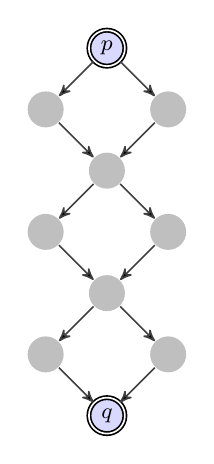
\begin{tikzpicture}[->,>=stealth',auto,node distance=1.1cm,
                    semithick,font=\footnotesize]

	\node[PRstate] (n0) {$p$};
	\node[state] (n1) [below left of=n0] {};
	\node[state] (n2) [below right of=n0] {};
	\node[state] (n3) [below right of=n1] {};
	\node[state] (n4) [below left of=n3] {};
	\node[state] (n5) [below right of=n3] {};
	\node[state] (n6) [below right of=n4] {};
	\node[state] (n7) [below left of=n6] {};
	\node[state] (n8) [below right of=n6] {};
	\node[PRstate] (n9) [below right of=n7] {$q$};

  \path [transition] 
		(n0) edge              node {} (n1);
  \path [transition] 
		(n0) edge              node {} (n2);
  \path [transition] 
		(n1) edge              node {} (n3);
  \path [transition] 
		(n2) edge              node {} (n3);
  \path [transition] 
		(n3) edge              node {} (n4);
  \path [transition] 
		(n3) edge              node {} (n5);
  \path [transition] 
		(n4) edge              node {} (n6);
  \path [transition] 
		(n5) edge              node {} (n6);
  \path [transition] 
		(n6) edge              node {} (n7);
  \path [transition] 
		(n6) edge              node {} (n8);
  \path [transition] 
		(n7) edge              node {} (n9);
  \path [transition] 
		(n8) edge              node {} (n9);
\end{tikzpicture}
\end{minipage} 
$\Longrightarrow$
\begin{minipage}[c]{.19\textwidth}
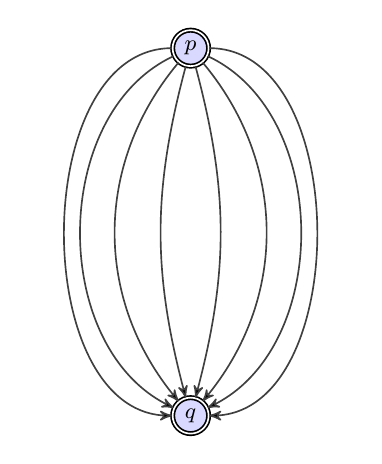
\begin{tikzpicture}[->,>=stealth',auto,node distance=1.1cm,
                    semithick,font=\footnotesize]

	\node[PRstate] (n0) {$p$};
	\node (n1) [below left of=n0] {};
	\node (n2) [below right of=n0] {};
	\node (n3) [below right of=n1] {};
	\node (n4) [below left of=n3] {};
	\node (n5) [below right of=n3] {};
	\node (n6) [below right of=n4] {};
	\node (n7) [below left of=n6] {};
	\node (n8) [below right of=n6] {};
	\node[PRstate] (n9) [below right of=n7] {$q$};

  \path [transition] 
		(n0) edge  [out=0, in=0]            node {} (n9);
  \path [transition] 
		(n0) edge  [out=180, in=180]        node {} (n9);
  \path [transition] 
		(n0) edge  [out=205, in=155]            node {} (n9);
  \path [transition] 
		(n0) edge  [out=230, in=130]            node {} (n9);
  \path [transition] 
		(n0) edge  [out=255, in=105]            node {} (n9);
  \path [transition] 
		(n0) edge  [out=-25, in=25]            node {} (n9);
  \path [transition] 
		(n0) edge  [out=-50, in=50]            node {} (n9);
  \path [transition] 
		(n0) edge  [out=-75, in=75]            node {} (n9);
\end{tikzpicture}
\end{minipage}
\caption{Expansion of the transition graph into a multigraph.}
\end{figure}

Classical interval analysis on this program yields $\lstinline|x_old| \in [-100000,100000]$. We have transformed the first program into the second, manually pruning out infeasible paths; yet in general the resulting program could be exponentially larger than the first (as in Fig.~\ref{fig:multigraph}), even though not all feasible paths are needed to compute the invariant. Following recent suggestions \cite{Gawlitza_Monniaux_ESOP11,Monniaux_Gonnord_SAS11}, we avoid this space explosion by keeping the second program implicit and working from the first program, yet simulating the analysis of the second program, that is, on a transition multigraph (Fig.~\ref{fig:multigraph}). Contribution \ref{contr:disjunctive} (\S\ref{sec:disjunctive}) replaces the exponential expansion of disjunctive invariant generation from \citet{DBLP:conf/pldi/GulwaniZ10} by an implicit representation; contribution \ref{contr:guided_multigraph} (\S\ref{sec:guided_multigraph}) recasts the ``guided analysis'' from \citet{DBLP:conf/sas/GopanR07} on an implicit representation of the paths in lieu of the individual transitions.

\section{Guided widening}
\label{sec:guided_multigraph}

\section{Disjunctive invariants}
\label{sec:disjunctive}

\section{Experimental comparisons}

\section{Conclusion}

% Cas a probleme:
% Initialisation (x,y) à {(1,0), (0,1)}
% puis boucle: si y = 0 alors x++
% fait un polyèdre qui finit par perdre y <= 1 et x >= 0

%\appendix
%\section{Appendix Title}

%This is the text of the appendix, if you need one.

%\acks

% Acknowledgments, if needed.

% We recommend abbrvnat bibliography style.
\bibliographystyle{dmabbrvnat}
\bibliography{implicitization}
\end{document}

% Pour Emacs:
% Local Variables:
% reftex-cite-format: natbib
% End:


\phantomsection\addcontentsline{toc}{section}{References} 
\bibliographystyle{splncs03}
\bibliography{implicitization}

\end{document}
